\documentclass[11pt]{article}
\usepackage[a4paper,margin=0.75in]{geometry}
\usepackage{amsmath,amssymb}
\usepackage{booktabs}
\usepackage{graphicx}
\usepackage[hidelinks]{hyperref}
\usepackage{enumitem}
\usepackage{tikz}
\usepackage{microtype}
\setlength{\emergencystretch}{4em}
\graphicspath{{../artifacts/figures/}}
\usetikzlibrary{arrows.meta,calc,positioning}

\newcommand{\src}[1]{\texttt{\footnotesize\detokenize{#1}}}

\begin{document}

\begin{center}
{\Large\bfseries 1D Ring and 2D Two-Target Bimodality Brief}\\[0.35em]
{\normalsize Focus: what was scanned, where double peaks appear, and which criteria should be used.}
\end{center}

\section*{1D Shortcut Ring}

\textbf{Reference configuration.}
Ring sites are labelled \(1,\ldots,N\). The reference case uses \(N=100\),
start \(n_0=1\), absorbing target \(51\), shortcut source
\(6=n_0+5\), and shortcut destination \(52=51+1\). Thus the shortcut is
one-way, \(6\to52\). Unless stated otherwise, \(q=2/3\), \(\rho=1\),
lazy\_selfloop, and the displayed reference case uses \(\beta=0.01\).

\begin{figure}[htbp]
\centering
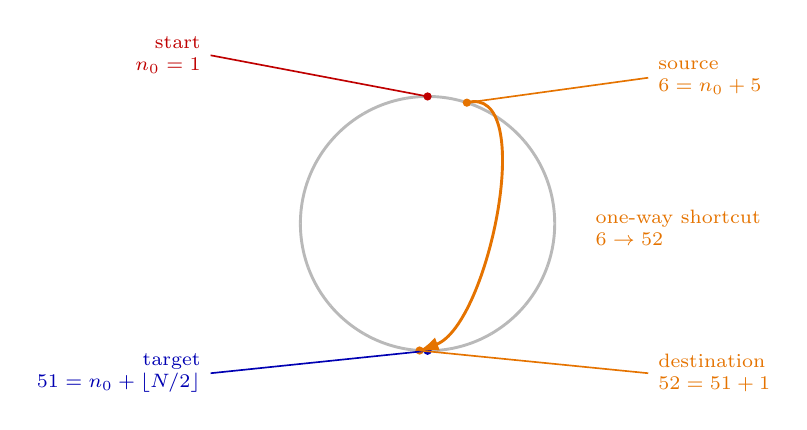
\begin{tikzpicture}[scale=0.95,every node/.style={font=\scriptsize}]
  \def\R{1.7}
  \coordinate (C) at (0,0);
  \coordinate (S0) at (90:\R);
  \coordinate (Src) at (72:\R);
  \coordinate (Target) at (-90:\R);
  \coordinate (Dst) at (-93.6:\R);
  \draw[gray!55,line width=1.05pt] (C) circle (\R);
  \foreach \ang in {0,20,...,340} {
    \fill[gray!45] (\ang:\R) circle (0.010);
  }
  \fill[red!75!black] (S0) circle (0.055);
  \fill[orange!90!black] (Src) circle (0.055);
  \fill[blue!70!black] (Target) circle (0.055);
  \fill[orange!90!black] (Dst) circle (0.055);

  \draw[red!75!black,line width=0.6pt] (S0) -- (-2.9,2.25)
    node[left,align=right] {start\\$n_0=1$};
  \draw[orange!90!black,line width=0.6pt] (Src) -- (2.95,1.95)
    node[right,align=left] {source\\$6=n_0+5$};
  \draw[blue!70!black,line width=0.6pt] (Target) -- (-2.9,-2.0)
    node[left,align=right] {target\\$51=n_0+\lfloor N/2\rfloor$};
  \draw[orange!90!black,line width=0.6pt] (Dst) -- (2.95,-2.0)
    node[right,align=left] {destination\\$52=51+1$};
  \draw[-{Latex[length=2.4mm]},orange!90!black,line width=1.05pt]
    (Src) to[out=15,in=20,looseness=0.75] (Dst);
  \node[orange!90!black,align=left] at (3.35,-0.05)
    {one-way shortcut\\$6\to52$};
\end{tikzpicture}

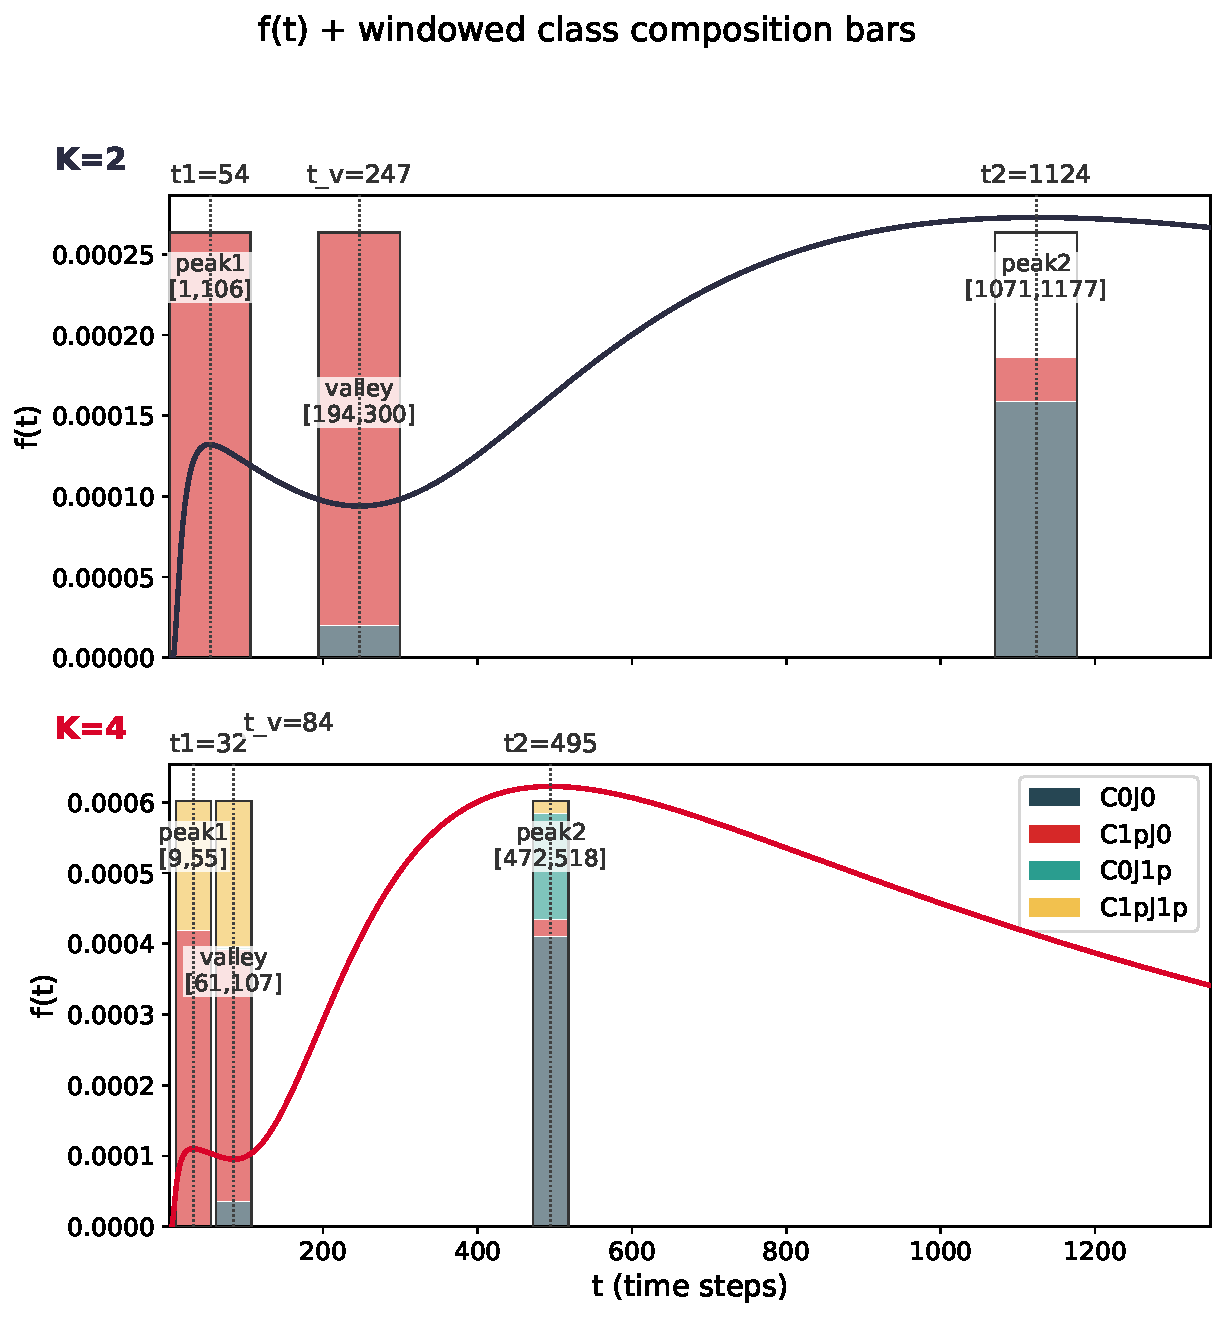
\includegraphics[width=0.92\linewidth]{shortcut_ring_k2_k4_beta001.pdf}
\caption{Reference configuration and first-passage curves at \(\beta=0.01\).
The early peak is shortcut-driven. The late peak is the slow non-shortcut
budget; for \(K=4\), jump-over/overshoot trajectories add a delayed component.}
\end{figure}

\section*{What Was Scanned}

\begin{table}[htbp]
\centering
\small
\begin{tabular}{p{0.24\linewidth}p{0.24\linewidth}p{0.21\linewidth}p{0.23\linewidth}}
\toprule
Scan & Parameters varied & Observed double-peak window & Readout \\
\midrule
Shortcut ring, fixed \(N=100\) &
\(\beta\) for \(K=2,4\); \(q=2/3\), \(\rho=1\), \(6\to52\) &
\(K=2:\ \beta=0.0005\)--\(0.05\);
\(K=4:\ \beta=0.001\)--\(0.15\) &
\(\beta=0\) gives no shortcut peak. Too-large \(\beta\) collapses the shape
toward an early shortcut-dominated peak. \\
\midrule
Shortcut ring, fixed \(\beta=0.02\) &
\(N=10,12,\ldots,200\), \(K=2,4\), antipodal target and shortcut just beyond target &
\(K=2:\ N\ge58\);
\(K=4:\ N\ge72\) &
Small rings do not separate the fast and slow timescales enough. Larger \(N\)
creates the late non-shortcut peak. \\
\midrule
Shortcut ring, fixed \(\beta=0.01\) &
\(N=50,52,\ldots,300\), \(K=2,4\) &
\(K=2:\ N\ge60\);
\(K=4:\ N\ge74\) &
The practical minimum size is roughly \(N\approx60\) for \(K=2\) and
\(N\approx70\)--\(75\) for \(K=4\). \\
\midrule
Two-target 1D ring &
\(L=31,51\), \(K=2\), drift \(g\in\{-0.6,-0.3,0,0.3,0.6\}\),
\(\beta\in\{0,0.03\}\), starts and two target locations &
34 classifier-confirmed \(\texttt{double\_peak}\) cases out of 240;
14 without shortcut, 20 with shortcut &
Double peaks can occur from target-channel competition alone. The shortcut
is helpful but not necessary. \\
\midrule
Two-target \(N\)-\(\beta\) scan &
\(N=30,35,\ldots,80\), \(\beta=0,0.01,\ldots,0.08\), \(K=2,4\) &
\(K=2:\ N=45\)--\(80\), \(\beta=0.01\)--\(0.08\);
\(K=4:\ N=50\)--\(80\), \(\beta=0.01\)--\(0.08\) &
The two-target mechanism needs enough spatial separation and a channel split;
otherwise the result is unimodal, shoulder, or local bump. \\
\bottomrule
\end{tabular}
\caption{Existing 1D ring scans already present in the repository.}
\end{table}

\section*{1D Ring Parameters That Decide the Shape}

\begin{table}[htbp]
\centering
\small
\begin{tabular}{p{0.20\linewidth}p{0.25\linewidth}p{0.45\linewidth}}
\toprule
Parameter & Values scanned or fixed & Effect on double peaks \\
\midrule
Ring size \(N\) or \(L\) &
\(N=10,\ldots,300\) in shortcut scans; \(L=31,51\) in two-target scans &
Controls timescale separation. Small rings merge the fast and slow budgets
into one peak. In the shortcut scan, visually useful double peaks start around
\(N\approx60\) for \(K=2\) and \(N\approx70\)--\(75\) for \(K=4\). \\
\midrule
Shortcut strength \(\beta\) &
\(\beta=0\) to \(0.15\) depending on scan &
Controls the mass in the fast shortcut channel. \(\beta=0\) removes the
shortcut peak. Too-large \(\beta\) overweights the early channel and weakens
the late peak. At \(N=100\), the observed window is roughly
\(\beta=0.0005\)--\(0.05\) for \(K=2\) and
\(\beta=0.001\)--\(0.15\) for \(K=4\). \\
\midrule
Jump range \(K\) &
\(K=2,4\) &
Controls path classes and overshoot/jump-over delays. \(K=4\) keeps
double peaks over a wider \(\beta\) interval because delayed non-shortcut or
overshoot trajectories remain visible. \\
\midrule
Shortcut placement &
Reference: \(6\to52\), target \(51\) &
Controls whether the shortcut creates a separate early arrival budget. If the
shortcut lands too close to the target or dominates too strongly, the late
budget can disappear as a visible second peak. \\
\midrule
Target locations and start &
Two-target ring scans over multiple starts and target pairs &
Controls target-channel competition. Double peaks can occur even without a
shortcut when one target contributes an early channel and the other contributes
a delayed channel. \\
\midrule
Drift \(g\) &
\(g\in\{-0.6,-0.3,0,0.3,0.6\}\) in the two-target ring scan &
Tilts probability mass toward one target channel. Moderate drift can improve
channel separation; strong drift can suppress one channel and turn the curve
into a single peak or shoulder. \\
\bottomrule
\end{tabular}
\caption{Concrete 1D parameters and what each one decides. The report should
claim \(\texttt{double\_peak}\) only when the classifier label supports it;
otherwise use shoulder or local bump.}
\end{table}

\begin{figure}[htbp]
\centering
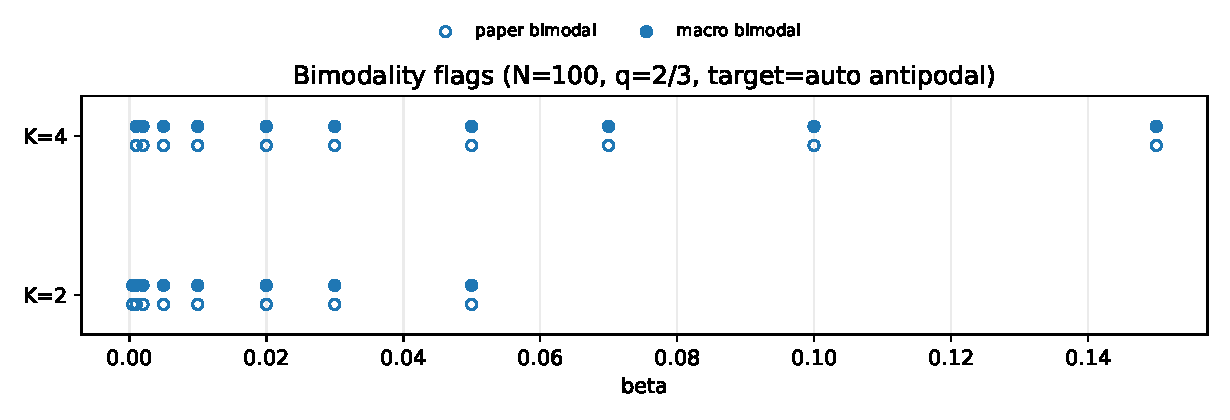
\includegraphics[width=0.49\linewidth]{shortcut_scan_beta_N100_bimodality.pdf}
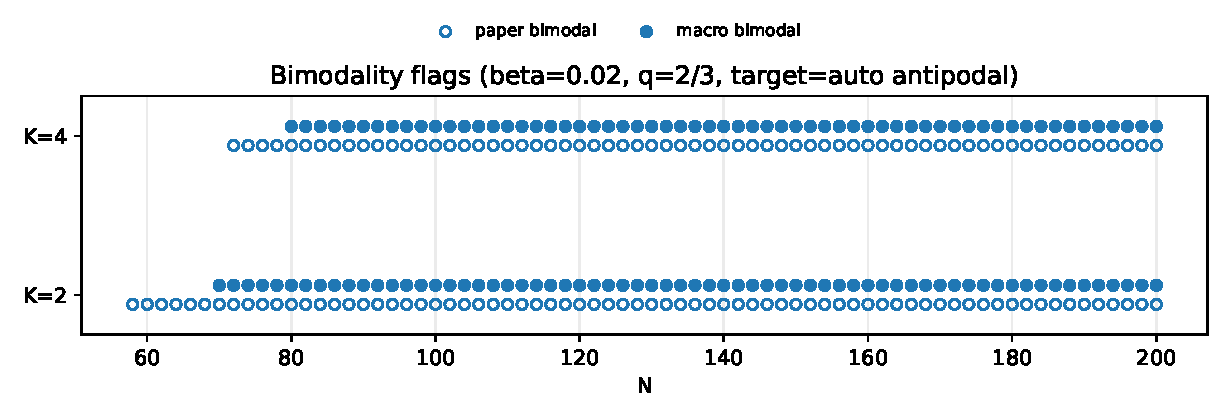
\includegraphics[width=0.49\linewidth]{shortcut_scan_N_beta002_bimodality.pdf}
\caption{Left: \(\beta\)-scan at \(N=100\). Right: \(N\)-scan at
\(\beta=0.02\). These figures show where the shortcut-ring classifier finds
two separated peaks.}
\end{figure}

\section*{2D Baseline Near/Far Target Bias-Radius Scan}

\textbf{Configuration.}
This part has also been done, but only as a bounded \(\theta=0\) slice rather
than a full angular scan. The grid is \(15\times9\), the start is fixed at
\((2,4)\), the far target is fixed at \((12,4)\), and the near target is placed
east of the start at radius \(r\). The boundary is reflecting
attempted-outside-stays. The global east bias moves probability mass from stay
to the east step:
\[
  p_E = q/4+b,\qquad p_N=p_S=p_W=q/4,\qquad p_{\mathrm{stay}}=1-q-b,
\]
with \(q=0.7\). The scan uses \(r=2,3,4,5\) and
\(b=0,0.04,0.08,0.12,0.16\), giving 20 cases.

The old radius-scan schematic is not used as the main configuration figure in
this brief. It is kept only as a baseline heatmap: a fixed-angle
\(\theta=0\) scan of near-target radius and global bias. The main 2D design
used below is the local-bias basin configuration.

\begin{table}[htbp]
\centering
\small
\begin{tabular}{p{0.24\linewidth}p{0.32\linewidth}p{0.34\linewidth}}
\toprule
Scan & Parameters varied & Readout \\
\midrule
2D near/far target, \(\theta=0\) &
\(r=2,3,4,5\), \(b=0,0.04,0.08,0.12,0.16\);
start \((2,4)\), far \((12,4)\) &
Double peaks appear when near-target hits and delayed far-target hits both
retain visible mass. Intermediate/strong east bias often helps, but distance
alone is not sufficient. \\
\bottomrule
\end{tabular}
\caption{Existing 2D bias-radius scan. Positive claims require the stored
classifier label to be exactly \(\texttt{double\_peak}\).}
\end{table}

\textbf{Classifier-confirmed 2D double-peak cases.}
The scan found 7 \(\texttt{double\_peak}\) cases out of 20:
\[
  (r,b)=(2,0.16),\ (3,0),\ (3,0.16),\ (4,0.08),\
  (4,0.12),\ (5,0.12),\ (5,0.16).
\]

\begin{figure}[htbp]
\centering
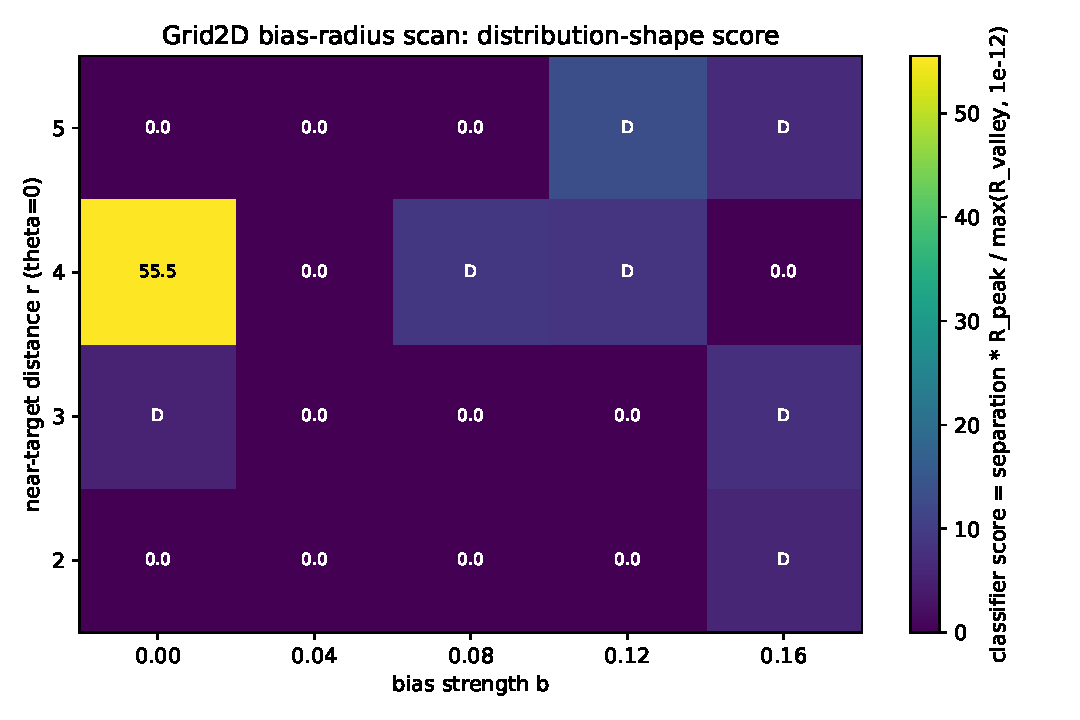
\includegraphics[width=0.72\linewidth]{grid2d_bias_radius_heatmap_theta0.pdf}
\caption{2D heatmap for the fixed \(\theta=0\) slice. Color is the classifier
score, not by itself a double-peak claim. The actual positive cases are the
seven rows labelled \(\texttt{double\_peak}\) in the metrics table.}
\end{figure}

\begin{figure}[htbp]
\centering
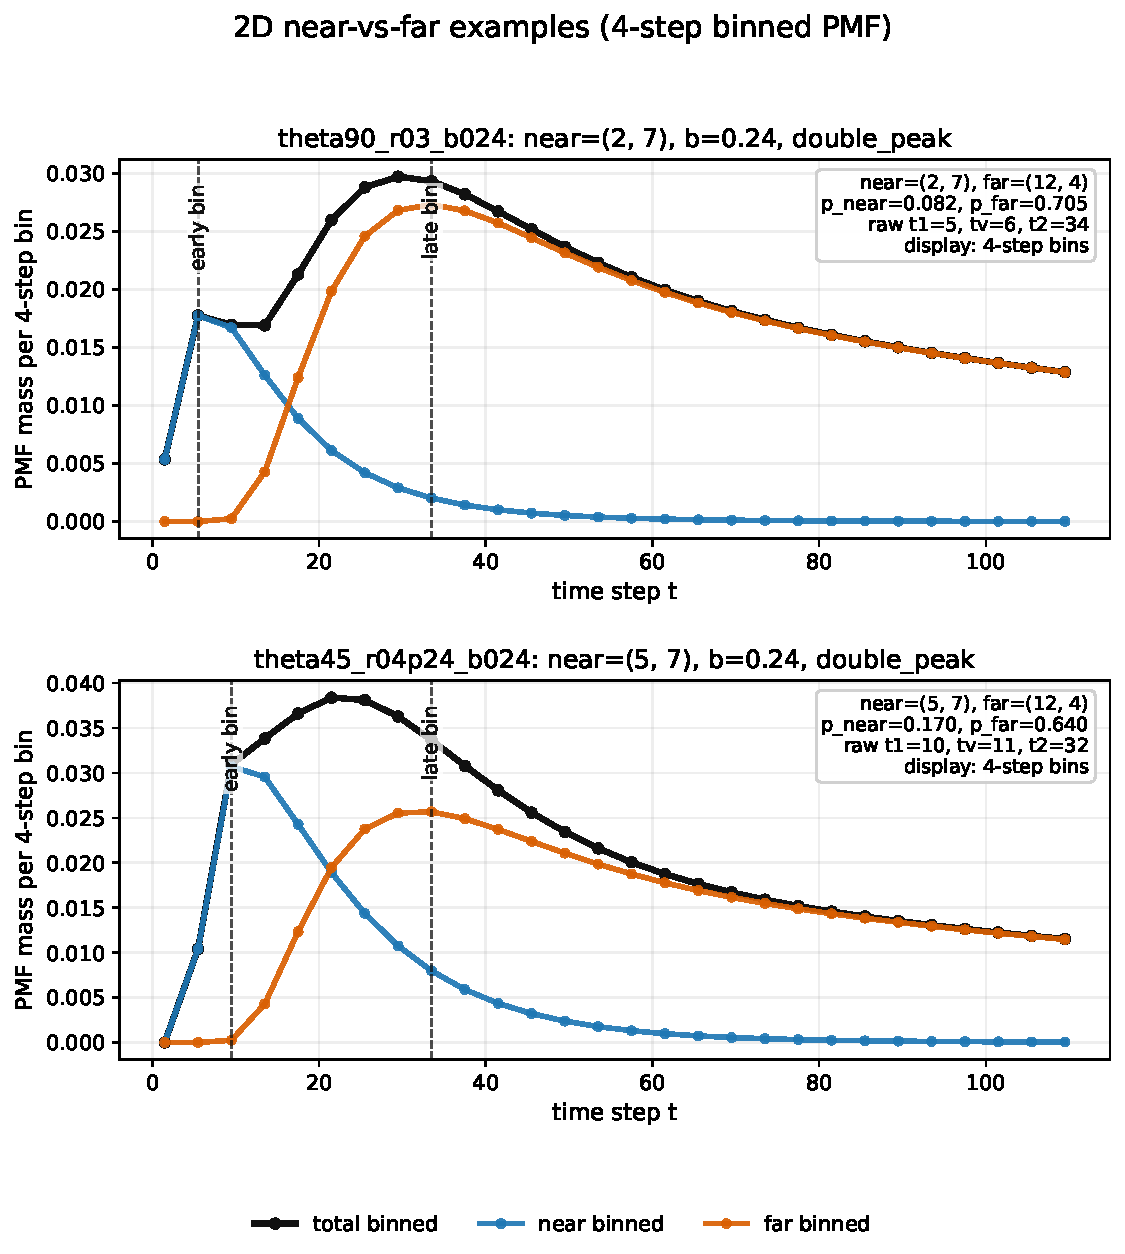
\includegraphics[width=0.92\linewidth]{grid2d_typical_double_peak_cases.pdf}
\caption{Two clearer 2D double-peak examples from a targeted \(\theta\)-expanded
search, displayed as 4-step binned probability mass for readability. The
classifier labels and peak times still come from the raw exact discrete-time
PMF. In both cases the near target is off the east-bias line, so the early peak
is a near-target channel and the late peak is dominated by delayed arrival at
the far target. These examples are illustrative, not a full angular phase
diagram.}
\end{figure}

\textbf{Why the display is binned.}
The exact computation gives a raw discrete-time PMF on a small grid, so the raw
curves contain parity and path-length oscillations, especially near the close
target. To avoid a jagged presentation figure, Figure 5 bins probability mass
into 4-step windows:
\[
  F_k=\sum_{t=4k}^{4k+3} f(t).
\]
This preserves probability mass and is only a display transform. The scientific
claims still use the raw classifier, raw peak times, and near/far channel
decomposition.

\section*{2D Main Configuration: Local-Bias Basin}

\textbf{Question.}
The fixed global-bias two-target scan can produce classifier-confirmed
\(\texttt{double\_peak}\) cases, but the visual shape is often weak because
the near target is hit by a small number of short paths. I therefore tested a
plain 2D rectangle with no corridor geometry, adding only a local bias basin
around the near target. The aim is to create a broader near-target residence
budget while keeping a delayed far-target budget alive.

\textbf{Configuration.}
The grid is a reflecting \(23\times13\) rectangle. The start is \((3,6)\), the
far target is \((19,6)\), and the far target is aligned with a global east
bias. The near target is moved off the east-bias line, e.g. \((5,9)\) or
\((5,3)\). Around the near target, a local basin of radius \(R_b\) is added.
Inside this basin there are two local effects:
\begin{enumerate}[leftmargin=1.5em,itemsep=0.2em]
\item a weak inward bias pointing toward the near target;
\item a local holding/slowing term that increases residence in the basin.
\end{enumerate}
Absorbing targets still take precedence: once either target is hit, the process
stops.

\begin{figure}[htbp]
\centering
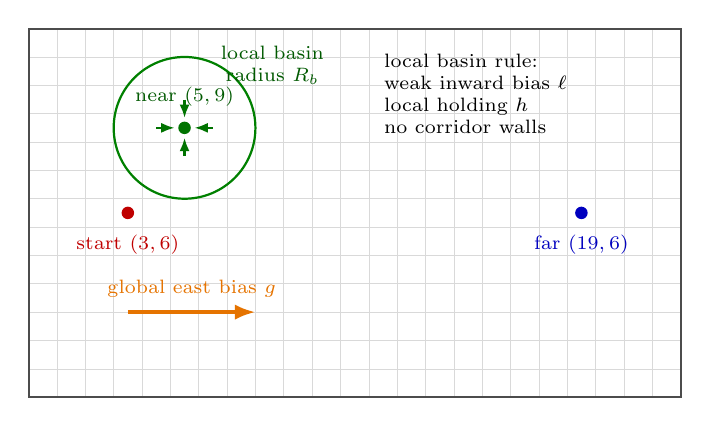
\begin{tikzpicture}[scale=0.36, every node/.style={font=\scriptsize}]
  \draw[step=1, gray!30, very thin] (0,0) grid (23,13);
  \draw[black!70, line width=0.7pt] (0,0) rectangle (23,13);
  \fill[red!75!black] (3.5,6.5) circle (0.22);
  \node[red!75!black, below] at (3.5,6.05) {start $(3,6)$};
  \fill[blue!75!black] (19.5,6.5) circle (0.22);
  \node[blue!75!black, below] at (19.5,6.05) {far $(19,6)$};
  \fill[green!45!black] (5.5,9.5) circle (0.22);
  \node[green!35!black, above] at (5.5,9.9) {near $(5,9)$};
  \draw[green!50!black, line width=0.8pt] (5.5,9.5) circle (2.5);
  \node[green!35!black, align=center] at (8.6,11.7) {local basin\\radius $R_b$};
  \draw[-{Latex[length=2.6mm]}, orange!90!black, line width=1.3pt] (3.5,3.0) -- (8.0,3.0);
  \node[orange!90!black, above] at (5.75,3.18) {global east bias $g$};
  \foreach \x/\y in {4.5/9.5,5.5/8.5,6.5/9.5,5.5/10.5} {
    \draw[-{Latex[length=1.7mm]}, green!45!black, line width=0.8pt] (\x,\y) -- ($(5.5,9.5)!0.35!(\x,\y)$);
  }
  \node[align=left, anchor=west] at (12.2,10.7)
    {local basin rule:\\weak inward bias $\ell$\\local holding $h$\\no corridor walls};
\end{tikzpicture}
\caption{Configuration for the local-bias basin test. The geometry remains a
plain reflecting rectangle. The added mechanism is a local near-target basin,
not a corridor.}
\end{figure}

\textbf{Small scan.}
The first local-bias scan used:
\[
  R_b\in\{2.5,3.5,4.5\},\quad
  g\in\{0.08,0.12,0.16,0.20\},\quad
  \ell\in\{0,0.04,0.08,0.12\},\quad
  h\in\{0,0.25,0.45\}.
\]
The near targets scanned were \((5,9),(7,9),(5,3),(7,3)\). This gives 576
cases. The raw exact PMF classifier found 210
\(\texttt{double\_peak}\) cases. Restricting to actual local inward bias
\(\ell>0\), it found 126 \(\texttt{double\_peak}\) cases.

\begin{table}[htbp]
\centering
\small
\begin{tabular}{p{0.18\linewidth}p{0.25\linewidth}p{0.47\linewidth}}
\toprule
Parameter & Values scanned or selected & Effect on the 2D shape \\
\midrule
Global east bias \(g\) &
\(0.08,0.12,0.16,0.20\); representative local-bias case uses \(g=0.16\) &
Keeps the far-target channel alive and shifts mass toward the delayed far
arrival. Too little global bias weakens the far-channel bump; too much can
overweight the far route and reduce near/far balance. \\
\midrule
Near-target position &
\((5,9),(7,9),(5,3),(7,3)\); best readable examples use \((5,9)\) or \((5,3)\) &
Moves the near target off the east-bias line. This prevents the near target
from absorbing the main eastward stream immediately and leaves enough mass for
the far target to form a delayed contribution. \\
\midrule
Basin radius \(R_b\) &
\(2.5,3.5,4.5\); representative local-bias case uses \(R_b=2.5\) &
Sets the size of the near-target capture region. A basin that is too small
looks like a short-path spike; a very broad basin can flatten the distinction.
The current local-bias-positive example works best at \(R_b=2.5\). \\
\midrule
Local inward bias \(\ell\) &
\(0,0.04,0.08,0.12\); representative local-bias case uses \(\ell=0.04\) &
Creates a weak capture drift toward the near target. Strong local attraction is
not ideal: it makes near absorption too fast and sharp. A weak value
\(\ell=0.04\) gives a clearer near channel while preserving the far channel. \\
\midrule
Local hold \(h\) &
\(0,0.25,0.45\); representative local-bias case uses \(h=0.25\) &
Broadens residence inside the near basin. This is the key smoothing mechanism:
it turns the near contribution from a short-path spike into a wider early
budget. \\
\midrule
Classifier and display &
Raw exact PMF for labels; 4-step binned mass for plots &
The \(\texttt{double\_peak}\) label is not assigned from the binned plot. The
binned plot only makes the discrete-time curve readable at report scale. \\
\bottomrule
\end{tabular}
\caption{Parameters that control the new 2D local-bias-basin configuration.
The strongest visual result is not strong local bias; it is weak capture plus
moderate local residence, while global bias maintains the delayed far channel.}
\end{table}

\begin{figure}[htbp]
\centering
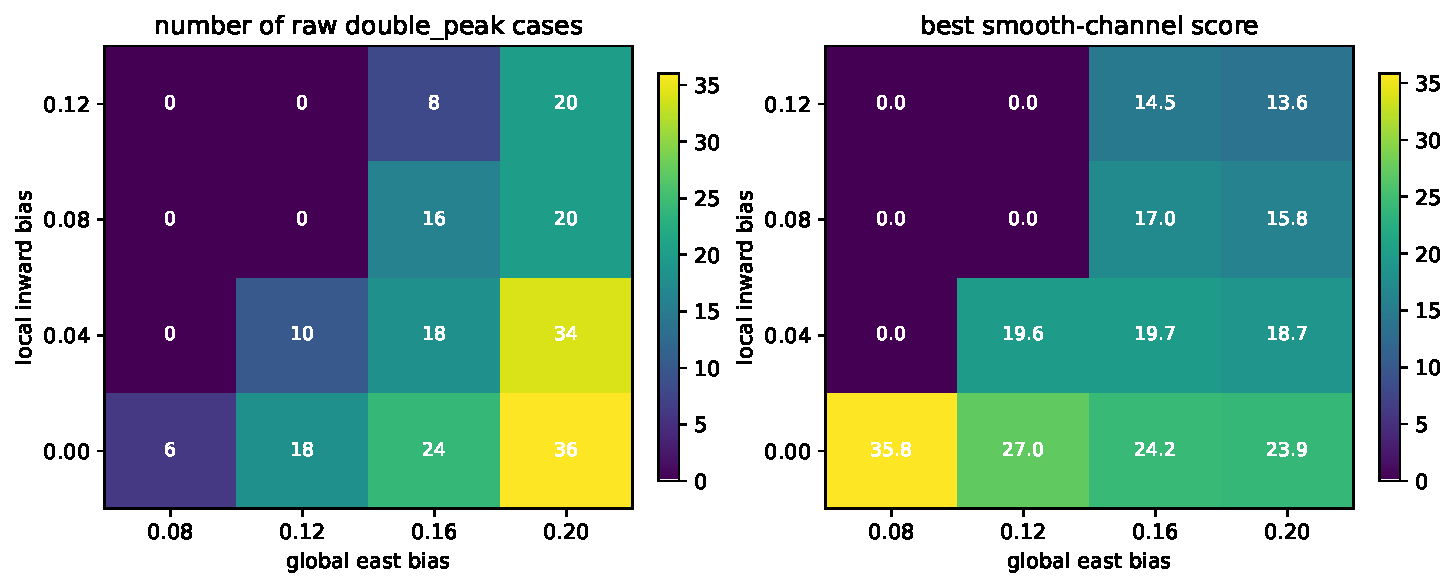
\includegraphics[width=0.86\linewidth]{grid2d_local_bias_basin_heatmap.pdf}
\caption{Local-bias basin scan. Left: number of raw classifier-confirmed
\(\texttt{double\_peak}\) cases aggregated over near-target position, basin
radius, and holding strength. Right: best smooth-channel score used to choose
readable examples.}
\end{figure}

\begin{figure}[htbp]
\centering
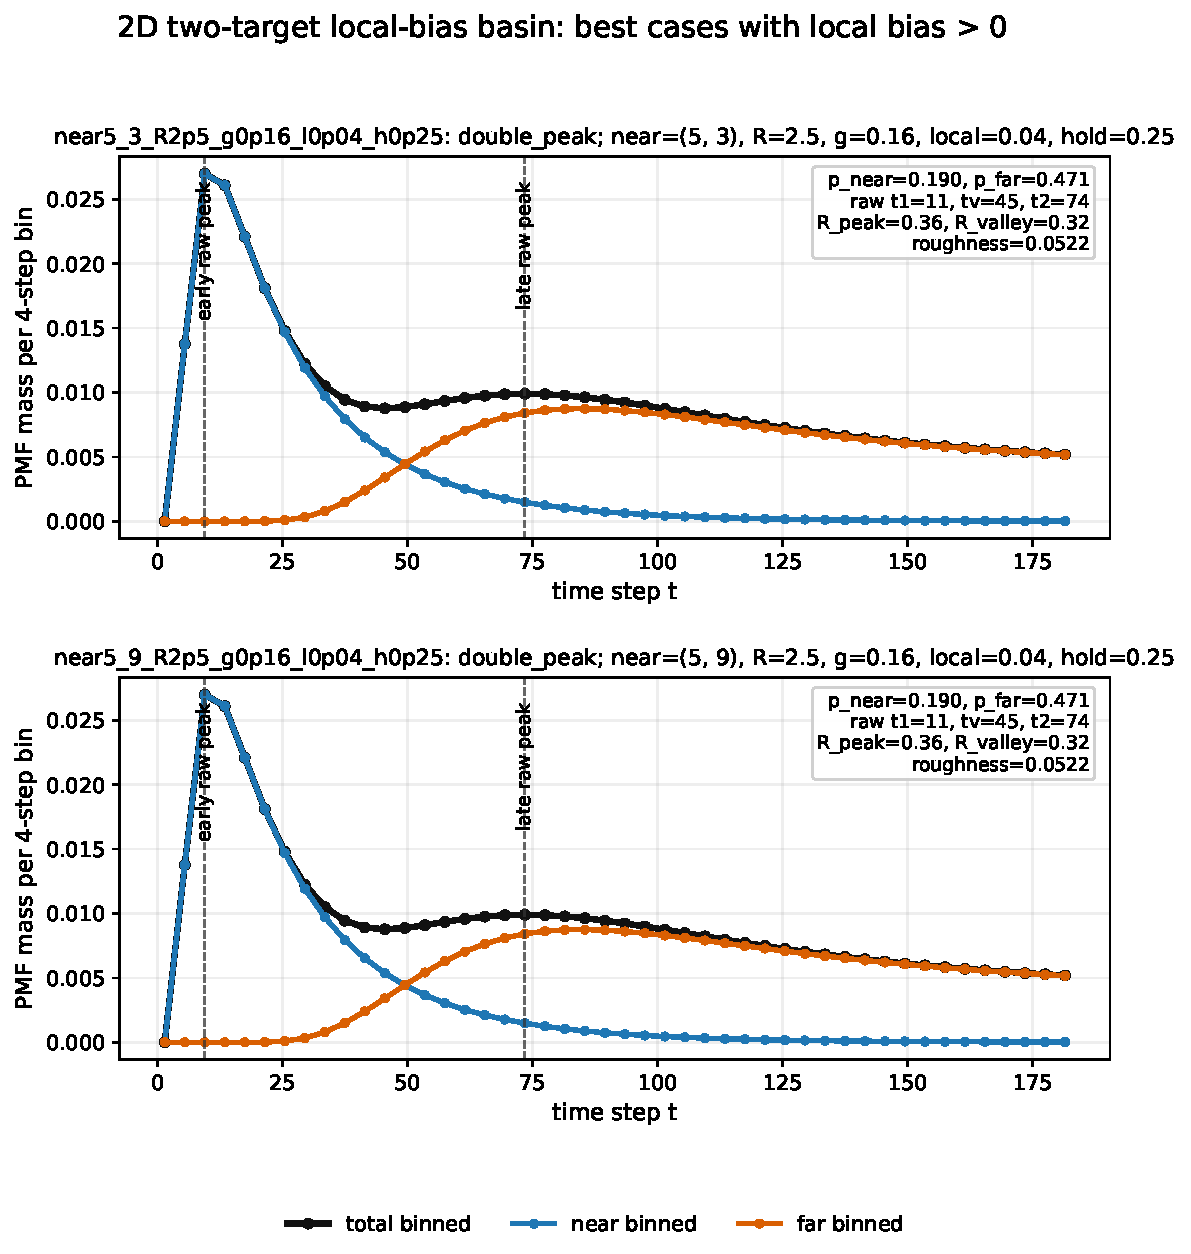
\includegraphics[width=0.92\linewidth]{grid2d_local_bias_basin_local_positive_best.pdf}
\caption{Best local-bias-positive examples, displayed as 4-step binned
probability mass. These are still classified using the raw exact PMF. A
representative setting is near \((5,3)\) or \((5,9)\), \(R_b=2.5\),
global east bias \(g=0.16\), local inward bias \(\ell=0.04\), and local hold
\(h=0.25\). The early peak is near-channel dominated, while the later broad
bump is far-channel dominated.}
\end{figure}

\textbf{Preliminary conclusion.}
The useful mechanism is not strong local attraction by itself. Strong local
bias tends to make near absorption too fast and sharp. The more promising
design is a weak local capture basin plus moderate local residence:
global east bias keeps the far-target channel alive, while the local basin
broadens the near-target contribution. This produces smoother two-target
double-peak-like curves without introducing corridor walls. This is still a
pilot scan, not a full 2D local-bias phase diagram.

\section*{Useful Double-Peak Criteria}

\textbf{Do not use ``two local maxima'' alone.}
That criterion is too permissive: it counts tiny numerical bumps and visually
weak shoulders. I would use a two-stage rule.

\begin{enumerate}[leftmargin=1.5em,itemsep=0.25em]
\item \textbf{Candidate screen:} two filtered local maxima above numerical
noise, with an inter-peak valley. This corresponds to the existing
\(\texttt{paper\_bimodal}\) or \(\texttt{double\_peak}\) classifier rows.
\item \textbf{Presentation claim:} report a double peak only when
\[
  t_2/t_1 \ge 10,\qquad h_2/h_1 \ge 0.05,\qquad
  h_v/\max(h_1,h_2) \le 0.6,
\]
and the peak pair has a mechanism explanation: shortcut/non-shortcut budget
split or target-channel split.
\item \textbf{Strict visual claim:} if the audience may challenge the shape,
use \(h_v/\max(h_1,h_2)\le0.3\). This is stricter and turns some weak
``double peak'' candidates into shoulders or local bumps.
\end{enumerate}

\begin{figure}[htbp]
\centering

\includegraphics[width=0.72\linewidth]{threshold_sweep_heatmap.pdf}
\caption{Threshold sensitivity scan. The scan varied the minimum peak height,
second-peak fraction, \(t_2/t_1\), and valley-depth threshold. This is why the
report should distinguish candidate bimodality from visually clear
bimodality.}
\end{figure}

\section*{What Helps or Blocks Double Peaks}

\textbf{Helps.}
Double peaks are easiest to see when the system creates two arrival budgets
with separated timescales. In the shortcut ring this is the fast shortcut
budget versus the slow non-shortcut budget. In the two-target ring this is the
near/early target channel versus the far/late target channel. In the 2D scan,
the same logic becomes a near-target channel versus a far-target channel under
eastward bias. In the new 2D local-bias design, global bias maintains the far
channel, while weak local capture plus local holding broadens the near-channel
budget.

\textbf{Blocks or weakens.}
Too small \(N\) compresses the two timescales into one peak. Too small
\(\beta\) removes the shortcut-driven early budget. Too large \(\beta\)
overweights the shortcut route and can erase the late component as a visible
second peak. In the two-target scan, weak channel separation gives shoulder or
local-bump labels rather than \(\texttt{double\_peak}\).
In the 2D scan, \(r=2\) needs stronger bias to show a labelled double peak,
while some larger-radius cases fail if the near and far channels do not both
remain visible.
The clearer near-vs-far examples found by the targeted \(\theta\)-expanded
search place the near target away from the east-bias line, e.g. near
\((2,7)\) or \((5,7)\) with \(b=0.24\). This lets the far target keep enough
probability mass to form a delayed second peak.

\textbf{Role of \(K\).}
For the shortcut ring, \(K=4\) is more robust over \(\beta\) than \(K=2\):
the sampled bimodal interval expands from \(\beta\le0.05\) for \(K=2\) to
\(\beta\le0.15\) for \(K=4\). The mechanism is that \(K=4\) has jump-over or
overshoot classes that add a delayed contribution to the slow side of the
distribution.

\section*{Older Shortcut Convention Kept Separate}

There is also an older shortcut convention for \(K=2\) with fixed shortcut
\(6\to56\) and target \(56\). That scan is useful as a threshold check, but it
is not the same as the current reference configuration \(6\to52\) with target
\(51\). Under the older \(6\to56\) convention,
\(\beta_c=2q/((1-q)N)=0.04\) is not an exact boundary for the existence of any
two local maxima, but it works as a practical boundary for visually meaningful
double peaks: above \(\beta_c\), the valley becomes too shallow for a clear
two-peak claim.

\section*{Source Files}

\begin{itemize}[leftmargin=1.5em,itemsep=0.2em]
\item Shortcut-ring beta and \(N\) scans:
\src{ring_lazy_jump_ext/artifacts/data/scan_beta_N100_K2.csv},
\src{scan_beta_N100_K4.csv}, \src{scan_N_K2_beta002.csv},
\src{scan_N_K4_beta002.csv}.
\item Larger \(N\)-scan at \(\beta=0.01\):
\src{ring_lazy_jump_ext/artifacts/outputs/N_sweep_beta_selected/}
\src{N_sweep_metrics_beta0.01.csv}.
\item Threshold sensitivity:
\src{ring_lazy_jump_ext_rev2/artifacts/outputs/sensitivity/threshold_sweep.csv}.
\item Two-target ring: \src{ring_two_target/artifacts/data/small_scan_metrics.csv},
\src{scan_bimodality_K2.csv}, and \src{scan_bimodality_K4.csv}.
\item 2D two-target bias-radius scan:
\src{grid2d_two_target_bias_radius/artifacts/data/grid2d_bias_radius_scan_metrics.csv},
\src{grid2d_double_peak_candidates.csv}, and
\src{grid2d_bias_radius_heatmap_theta0.pdf}.
\item 2D targeted examples:
\src{final_multitimescale_fpt_encounter/artifacts/data/grid2d_typical_double_peak_cases.csv}
and \src{grid2d_typical_double_peak_cases.pdf}.
\item 2D local-bias basin pilot:
\src{final_multitimescale_fpt_encounter/code/scan_grid2d_local_bias_basin.py},
\src{final_multitimescale_fpt_encounter/artifacts/data/grid2d_local_bias_basin_scan.csv},
\src{grid2d_local_bias_basin_heatmap.pdf}, and
\src{grid2d_local_bias_basin_local_positive_best.pdf}.
\end{itemize}

\end{document}
